%\newpage
\section{NURBS parametrization of the sphere}
Two standard ways of parameterizing a sphere using NURBS are given below for the unit sphere (a simple scaling generalizes this for spheres of arbitrary radii). The first is represented by 8 elements in a single patch (only one element is given below, as the others are obtained by symmetry), and the second is represented by 6 patches (only one patch is given below, as the others are obtained by symmetry).
\subsection{Parametrization 1}
\label{Sec3:NURBSsphere1}
The sphere can be exactly parameterized by 8 NURBS elements of degree 2. One of these elements with corresponding control points are illustrated in \Cref{Fig3:parametrizationOfSphere1}. The weights and control points are given in \Cref{Tab3:sphere1} (a parametrization of all elements in a single patch can be found in~\cite[p. 168]{Venas2015iao}).
\begin{figure}
	\centering
	\begin{subfigure}{0.40\textwidth}
		\centering
%		\includegraphics[width=0.9\textwidth]{\graphicsFolder/Figure37a}
		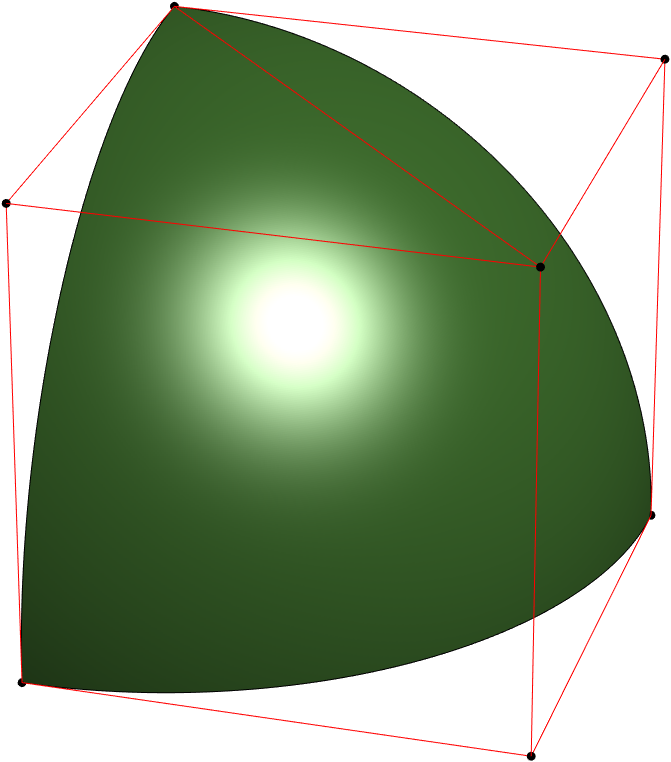
\includegraphics[width=0.9\textwidth]{../../graphics/sphericalShell/Sphere1controlPolygon}
		\caption{Parametrization 1}
		\label{Fig3:parametrizationOfSphere1} 
	\end{subfigure}
	~
	\begin{subfigure}{0.55\textwidth}
		\centering
%		\includegraphics[width=0.9\textwidth]{\graphicsFolder/Figure37b}
		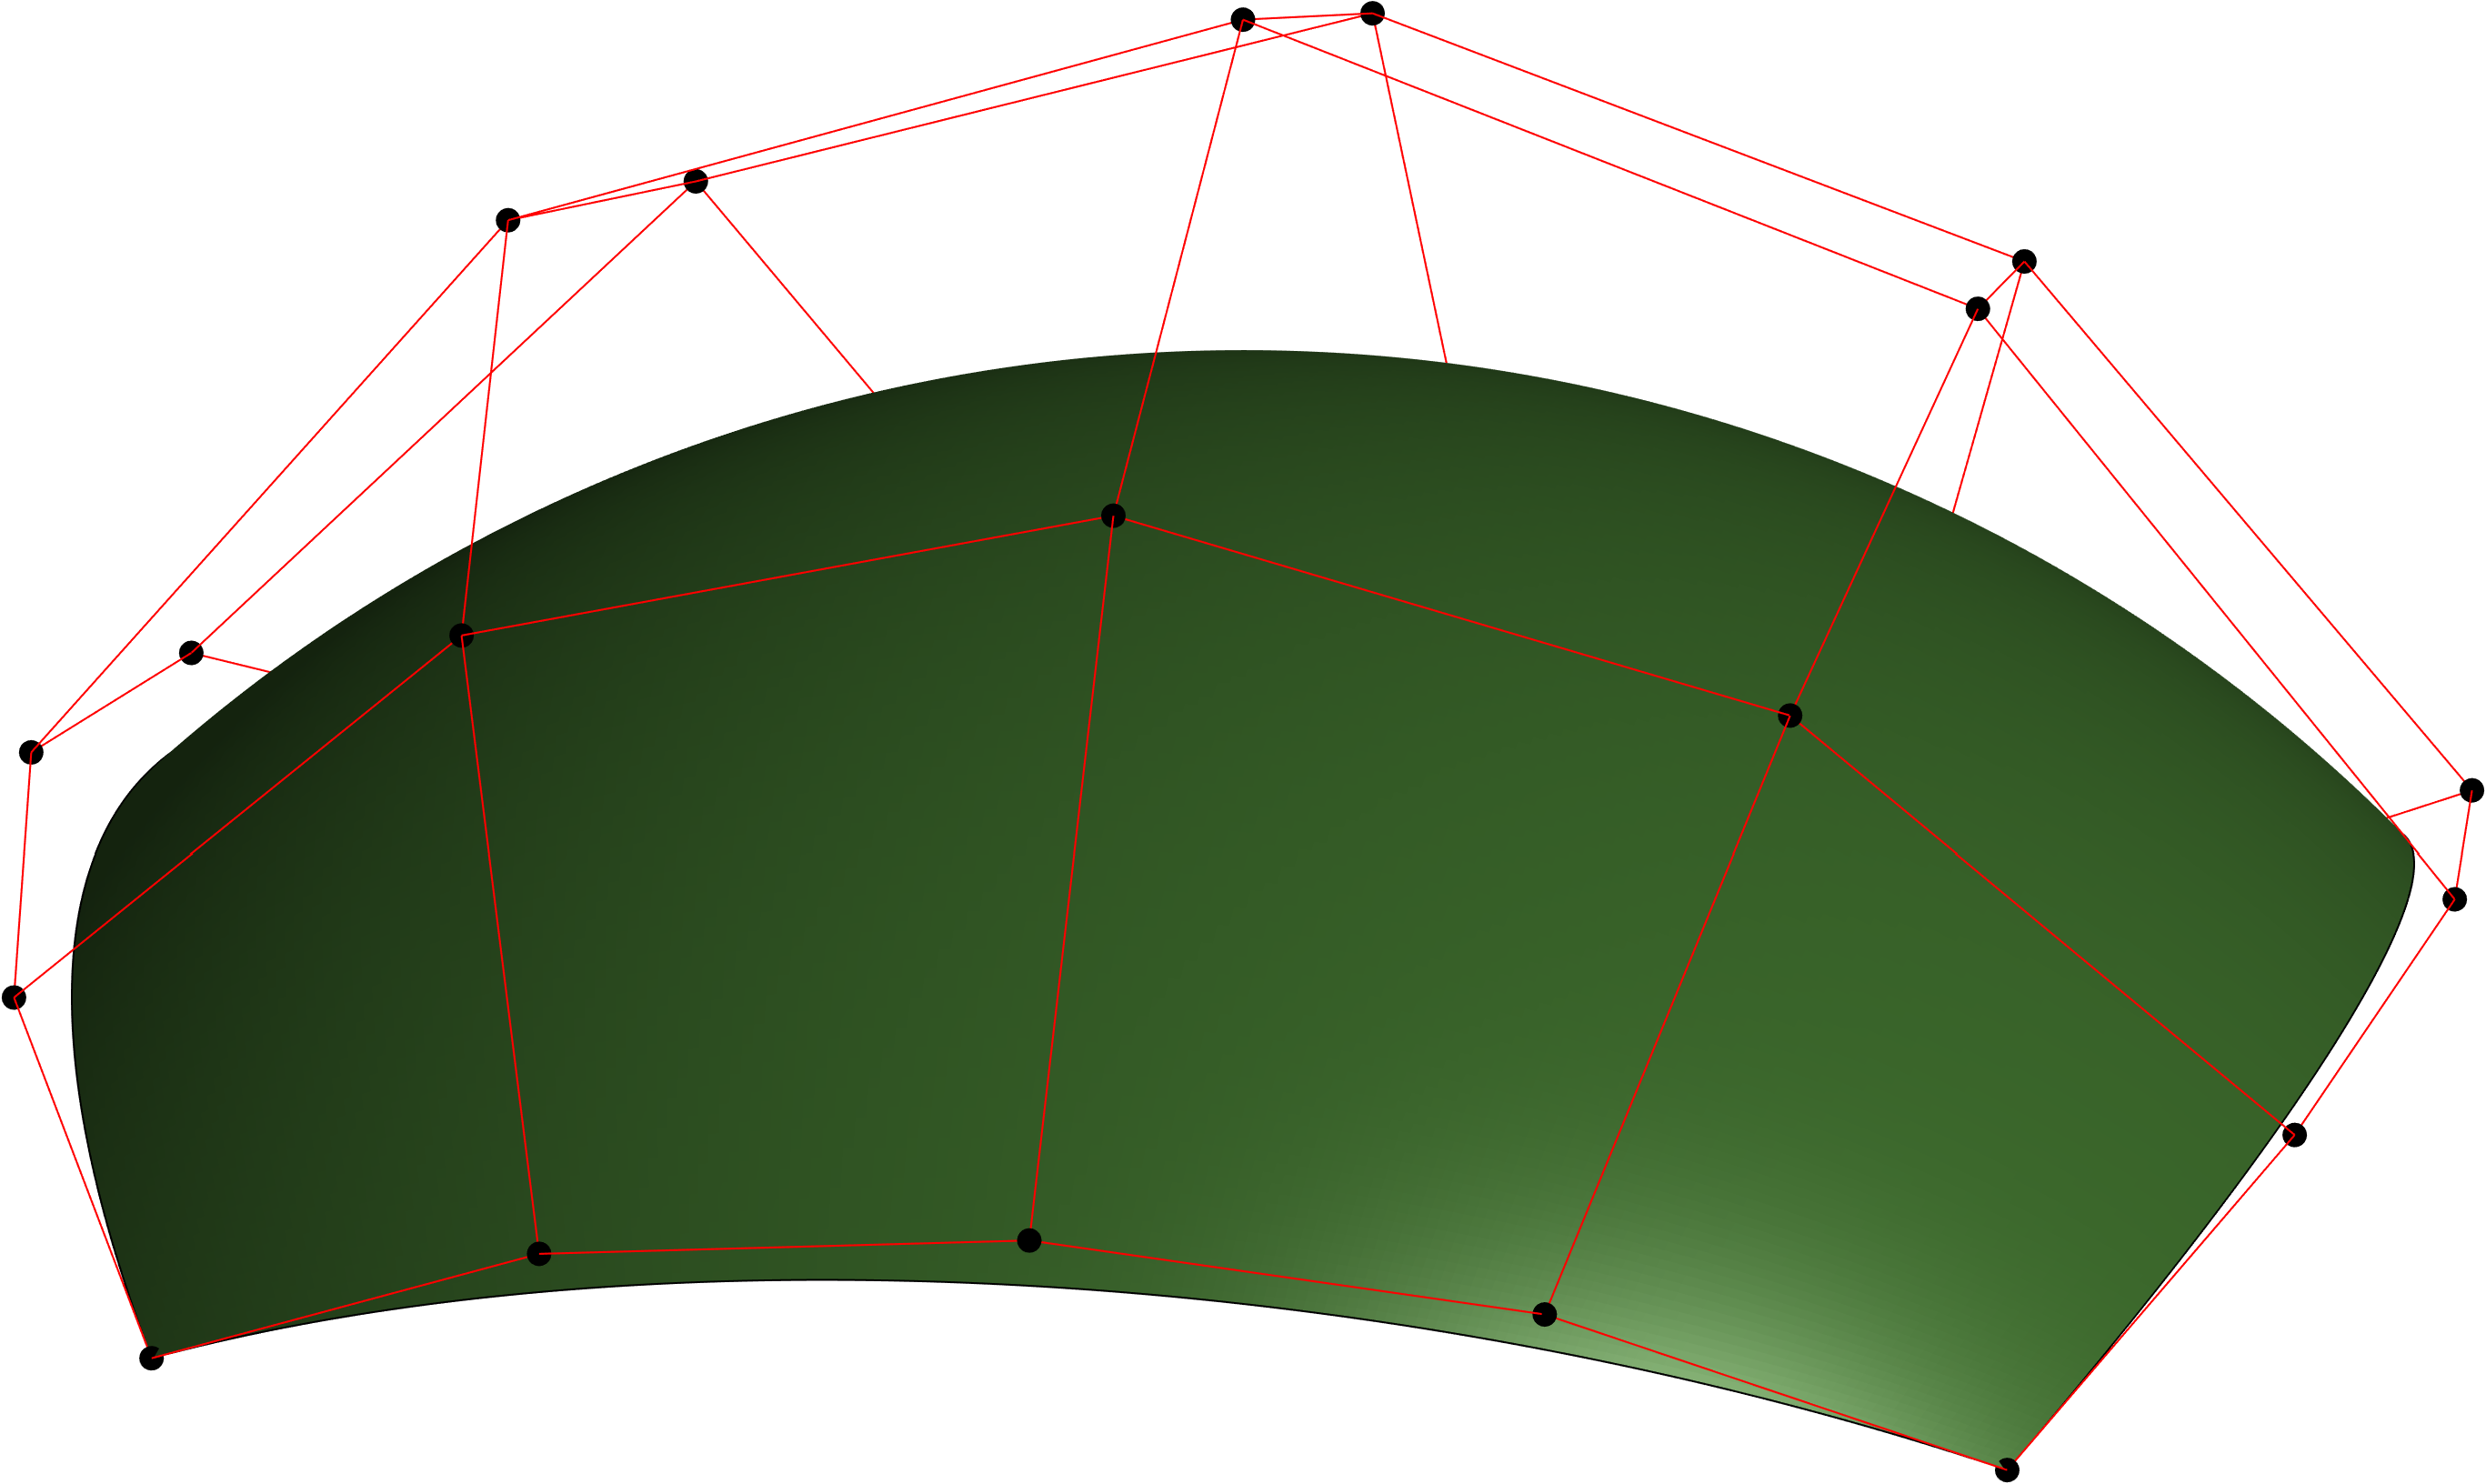
\includegraphics[width=0.9\textwidth]{../../graphics/MA8502/Sphere2controlPolygon}
		\caption{Parametrization 2}
		\label{Fig3:parametrizationOfSphere2} 
	\end{subfigure}
	\caption{\textbf{NURBS parametrization of the sphere}: Two NURBS parametrizations of the sphere. The control polygon is also shown.}       
\end{figure}

\begin{table}
	\centering
	\caption{\textbf{Parametrization 1}: Weights and control points for an element of a unit sphere.}
	\label{Tab3:sphere1}
	\begin{tabular}{c c c c c c}
		\toprule
		$i$		& 	$j$	& 	$x_{i,j}$ 	& $y_{i,j}$ 	& $z_{i,j}$ 	& $w_{i,j}$\\
		\hline
		$1$		&	$1$	&	1	& 0		& 0		&	1				\\
		$2$		&	$1$	&	1	& 1		& 0 	&	$1/\sqrt{2}$	\\
		$3$		&	$1$	&	0	& 1		& 0		&	1				\\ \\
		
		$1$		&	$2$	&	1	& 0		& 1		&	$1/\sqrt{2}$				\\
		$2$		&	$2$	&	1	& 1		& 1 	&	$1/2$	\\
		$3$		&	$2$	&	0	& 1		& 1		&	$1/\sqrt{2}$				\\ \\
		
		$1$		&	$3$	&	0	& 0		& 1		&	1				\\
		$2$		&	$3$	&	0	& 0		& 1 	&	$1/\sqrt{2}$	\\
		$3$		&	$3$	&	0	& 0		& 1		&	1				\\
		\bottomrule
	\end{tabular}
\end{table}

\subsection{Parametrization 2}
\label{Sec3:NURBSsphere2}
The sphere can be exactly parameterized \cite[p. 11]{Cobb1988tts} by 6 NURBS patches of degree 4. One of these patches with corresponding control points are illustrated in \Cref{Fig3:parametrizationOfSphere2}. Some of the weights and weighted control points are given in \Cref{Tab3:sphere2}. The remaining data is found by symmetry about the planes $x=0$, $y=0$, $y=x$ and $y=-x$. In particular (by symmetry about the $y=x$ plane)
\begin{equation*}
	x_{i,j} = y_{j,i},\quad y_{i,j} = x_{j,i},\quad z_{i,j} = z_{j,i},\quad w_{i,j} = w_{j,i}
\end{equation*}
for the pairs $(i,j) \in\{(1,2),(1,3),(2,3)\}$, and (by symmetry about the $y=0$ plane)
\begin{equation*}
	x_{i,j} = -x_{6-i,j},\quad y_{i,j} = y_{6-i,j},\quad z_{i,j} = z_{6-i,j},\quad w_{i,j} = w_{6-i,j}
\end{equation*}
for $i=4,5$ and $j=1,2,3$, and then (by symmetry about the $x=0$ plane)
\begin{equation*}
	x_{i,j} = x_{i,6-j},\quad y_{i,j} = -y_{i,6-j},\quad z_{i,j} = z_{i,6-j},\quad w_{i,j} = w_{i,6-j}
\end{equation*}
for $i=1,2,3,4,5$ and $j=4,5$.

\begin{table}
	\centering
	\caption{\textbf{Parametrization 2}: Weights and weighted control points for a tile of a unit sphere.}
	\label{Tab3:sphere2}
	\begin{tabular}{c c c c c c}
		\toprule
		$i$		& 	$j$	& 	$w_{i,j}x_{i,j}$ 	& $w_{i,j}y_{i,j}$ 	& $w_{i,j}z_{i,j}$ 	& $w_{i,j}$\\
		\hline
		$1$		&	$1$	&	$4(1-\sqrt{3})$ 	& $4(1-\sqrt{3})$ 			& $4(\sqrt{3}-1)$		&	$4(3-\sqrt{3})$				\\
		$2$		&	$1$	&	$-\sqrt{2}$ 		& $\sqrt{2}(\sqrt{3}-4)$ 	& $\sqrt{2}(4-\sqrt{3})$&	$\sqrt{2}(3\sqrt{3}-2)$				\\
		$3$		&	$1$	&	$0$ 				& $4(1-2\sqrt{3})/3$ 		& $ 4(2\sqrt{3}-1)/3$	&	$4(5-\sqrt{3})/3$				\\ \\
		
		
		$2$		&	$2$	&	$-(3\sqrt{3}-2)/2$ 	& $(2-3\sqrt{3})/2$ 		& $(\sqrt{3}+6)/2$		&	$(\sqrt{3}+6)/2$				\\
		$3$		&	$2$	&	$0$ 				& $\sqrt{2}(2\sqrt{3}-7)/3$ & $5\sqrt{6}/3$		&	$\sqrt{2}(\sqrt{3}+6)/3$\\ \\
		
		
		$3$		&	$3$	&	$0$ 				& $0$ 						& $4(5-\sqrt{3})/3$		&	$4(5\sqrt{3}-1)/9$				\\
		\bottomrule
	\end{tabular}
\end{table}

\section{NURBS parametrization of the torus}
\label{Sec3:torus}
A torus with major radius $r_{\mathrm{o}}$ and minor radius $r_{\mathrm{i}}$ can be represented by a single NURBS patch with 16 elements (as visualized in \Cref{Fig3:Torus}). One of these elements are shown in~\Cref{Fig3:parametrizationOfTorus} with corresponding control polygon. The weights and control points are given in \Cref{Tab3:torus}.
\begin{figure}
	\centering
%	\includegraphics[width=0.7\textwidth]{\graphicsFolder/Figure38}
	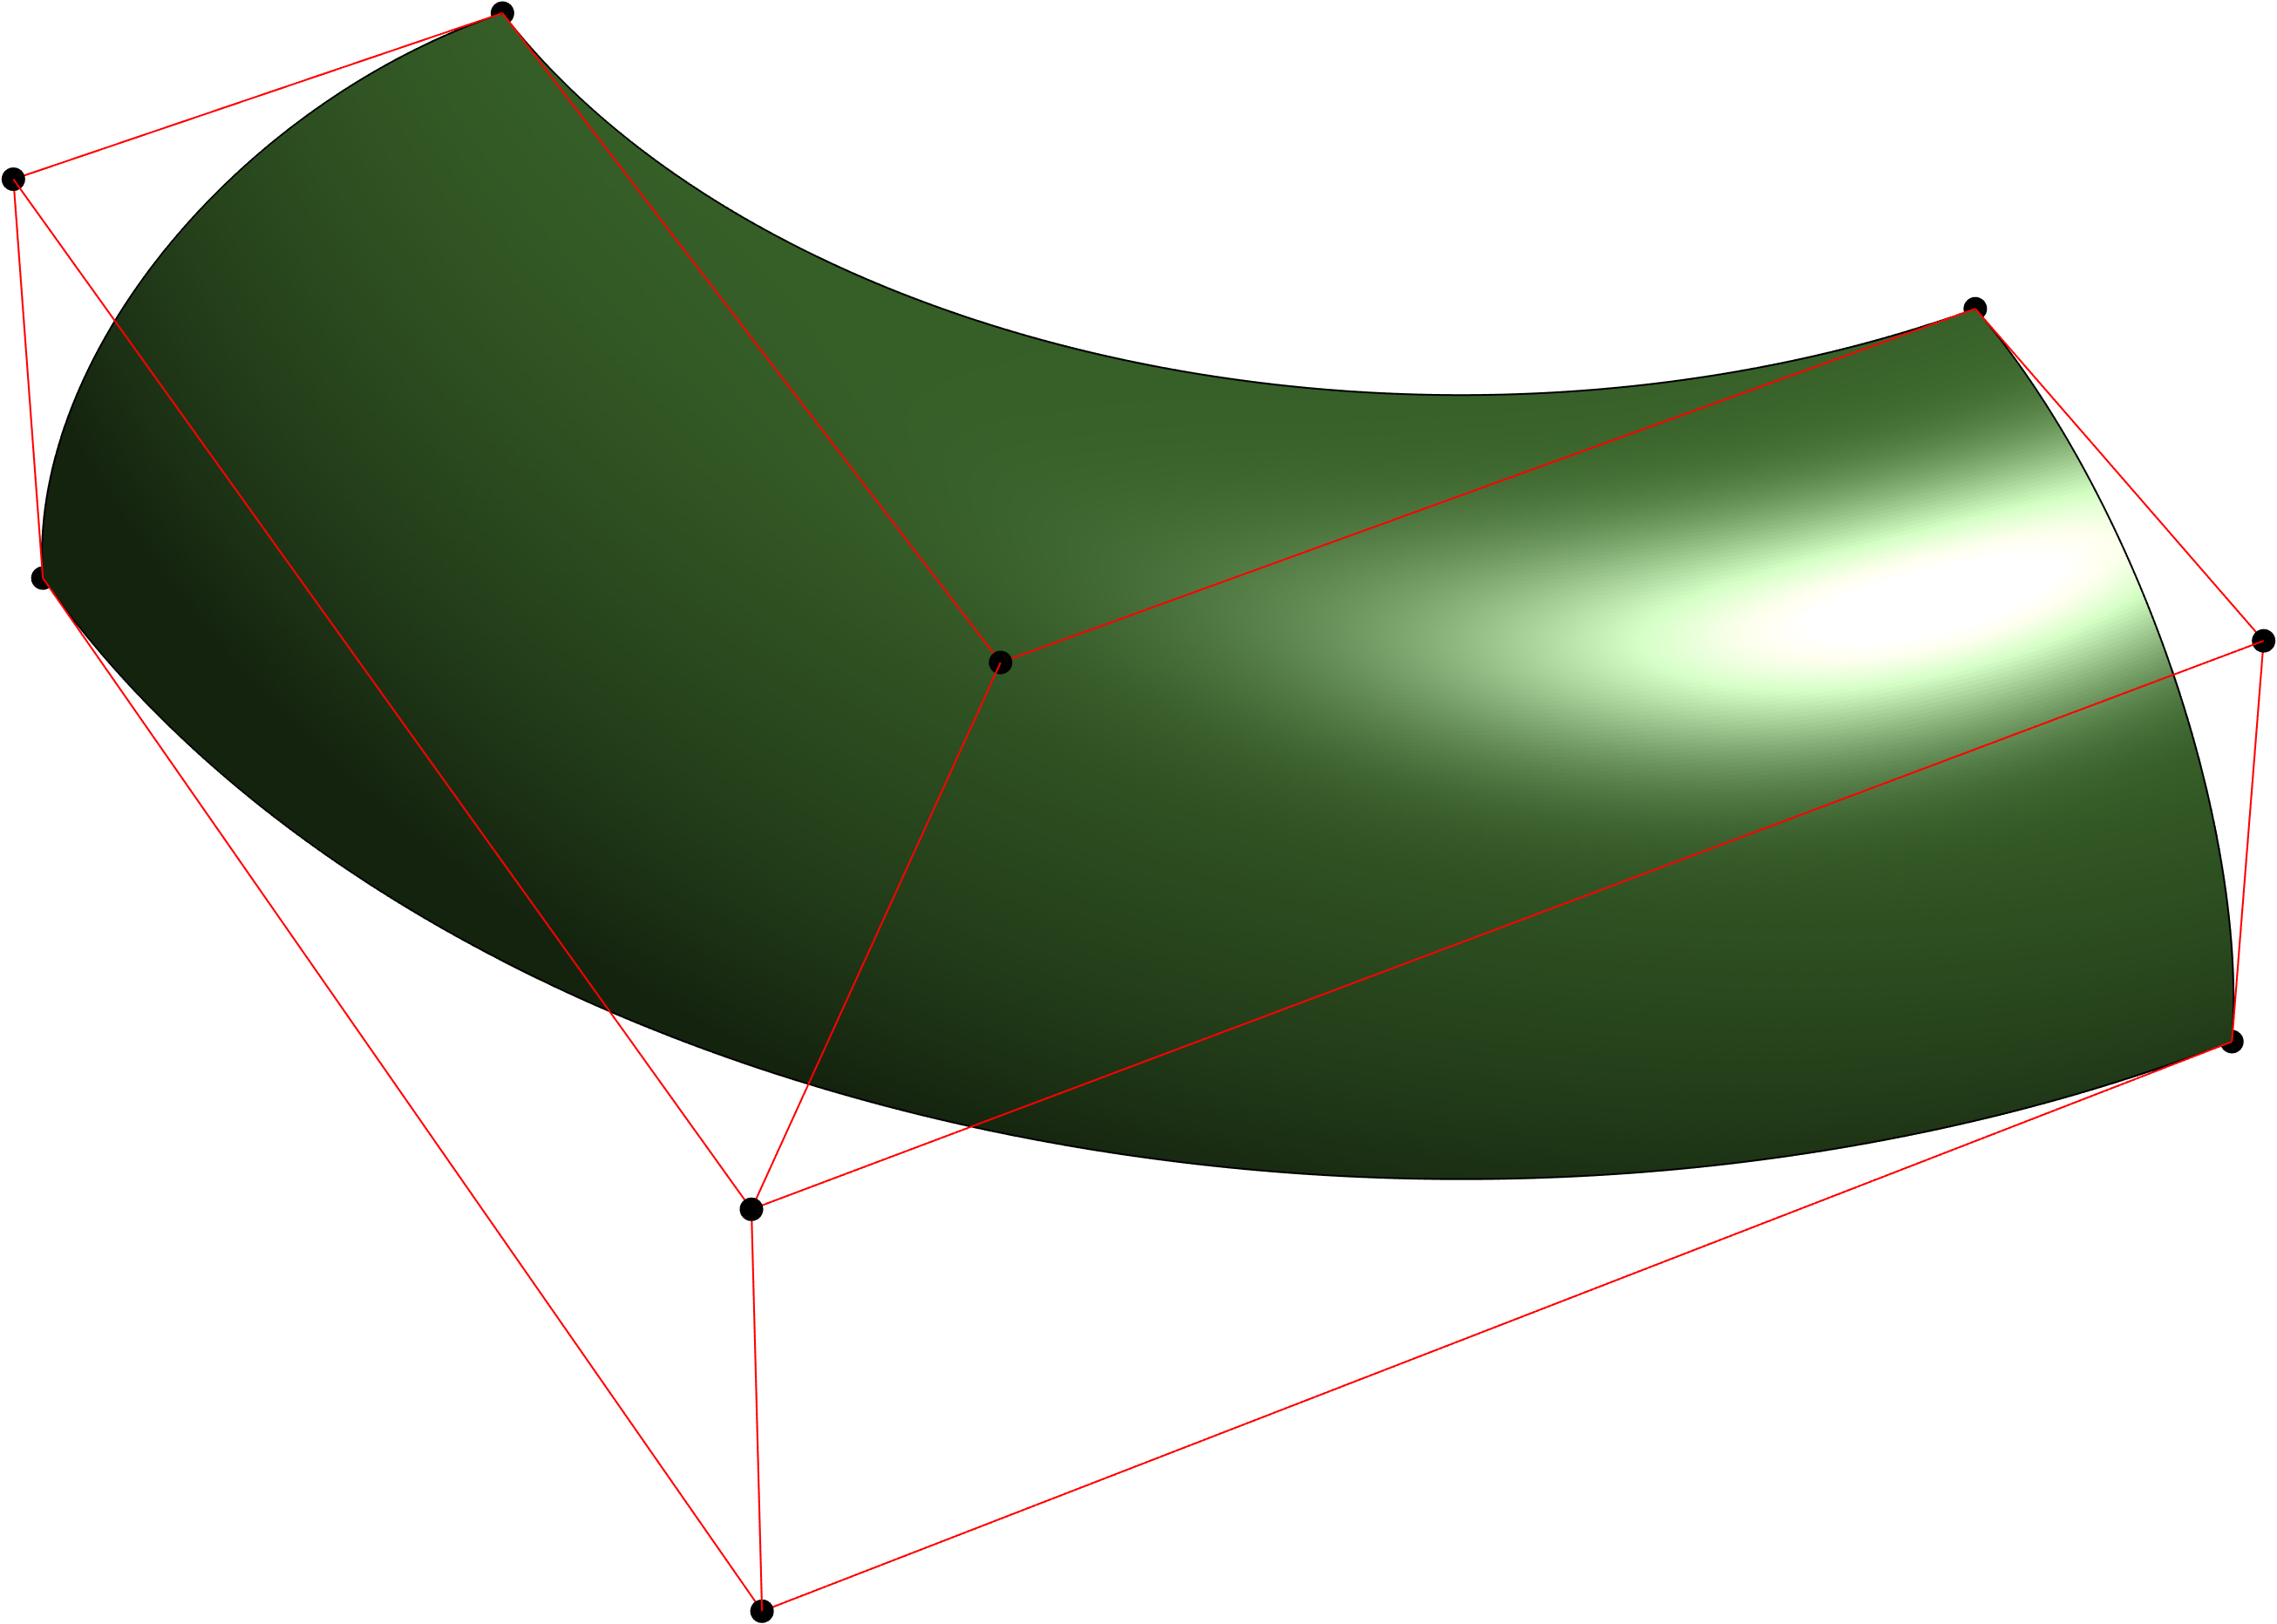
\includegraphics[width=0.7\textwidth]{../../graphics/TorusControlPts}
	\caption{\textbf{NURBS parametrization of the torus}: A NURBS parametrizations of a 1/16 of a torus. The control polygon is also shown.}       
	\label{Fig3:parametrizationOfTorus} 
\end{figure}

\begin{table}
	\centering
	\caption{\textbf{NURBS parametrization of the torus}: Weights and control points for the torus.}
	\label{Tab3:torus}
	\begin{tabular}{c c c c c c}
		\toprule
		$i$		& 	$j$	& 	$x_{i,j}$ 	& $y_{i,j}$ 	& $z_{i,j}$ 	& $w_{i,j}$\\
		\hline
		$1$		&	$1$	&	$r_{\mathrm{o}}+r_{\mathrm{i}}$	& 0		& 0		&	1				\\
		$2$		&	$1$	&	$r_{\mathrm{o}}+r_{\mathrm{i}}$	& $r_{\mathrm{o}}+r_{\mathrm{i}}$		& 0 	&	$1/\sqrt{2}$	\\
		$3$		&	$1$	&	0	& $r_{\mathrm{o}}+r_{\mathrm{i}}$		& 0		&	1				\\ \\
		
		$1$		&	$2$	&	$r_{\mathrm{o}}+r_{\mathrm{i}}$	& 0		& $r_{\mathrm{i}}$		&	$1/\sqrt{2}$				\\
		$2$		&	$2$	&	$r_{\mathrm{o}}+r_{\mathrm{i}}$	& $r_{\mathrm{o}}+r_{\mathrm{i}}$		& $r_{\mathrm{i}}$ 	&	$1/2$	\\
		$3$		&	$2$	&	0	& $r_{\mathrm{o}}+r_{\mathrm{i}}$		& $r_{\mathrm{i}}$		&	$1/\sqrt{2}$				\\ \\
		
		$1$		&	$3$	&	$r_{\mathrm{o}}$	& 0		& $r_{\mathrm{i}}$		&	1				\\
		$2$		&	$3$	&	$r_{\mathrm{o}}$	& $r_{\mathrm{o}}$		& $r_{\mathrm{i}}$ 	&	$1/\sqrt{2}$	\\
		$3$		&	$3$	&	0	& $r_{\mathrm{o}}$	& $r_{\mathrm{i}}$		&	1				\\
		\bottomrule
	\end{tabular}
\end{table}